\chapter{Project Analysis}\glsresetall
\section{The Spatial Stokes Layer (SSL) Mean Velocity Profile}\label{sec:sslmean}
Since we do not know the shape of the \gls{ww} mean streamwise velocity profile to figure out dissipation due to the mean profile, we must start elsewhere. The \gls{ssl} mean streamwise velocity profile $\overline{U}\ssl\ps$ was given by \vqt, along with that of \gls{tsl}, the reference channel flow, and $\overline{U}^{+}=y^{+}$ for comparison (Figure~\ref{fig:sslmeanprofile}). We can see that at $y^{+}<10$, they all coincide to the linear profile $\overline{U}^{+}=y^{+}$, and at some point between $10<y^{+}<40$, they stop being curved on the logarithmic plot and become straight with similar slopes, indicating a logarithmic profile at higher $y^{+}$. In fact, like other \gls{dr} techniques (e.g. riblets), the \gls{dr} is noticeable as a thickening of the viscous sublayer causing an upward shift in this logarithmic portion of the mean velocity profile \cite{viotti2009,choi1989,luchini1996}. 

\begin{figure}[htbp]
	\centering
	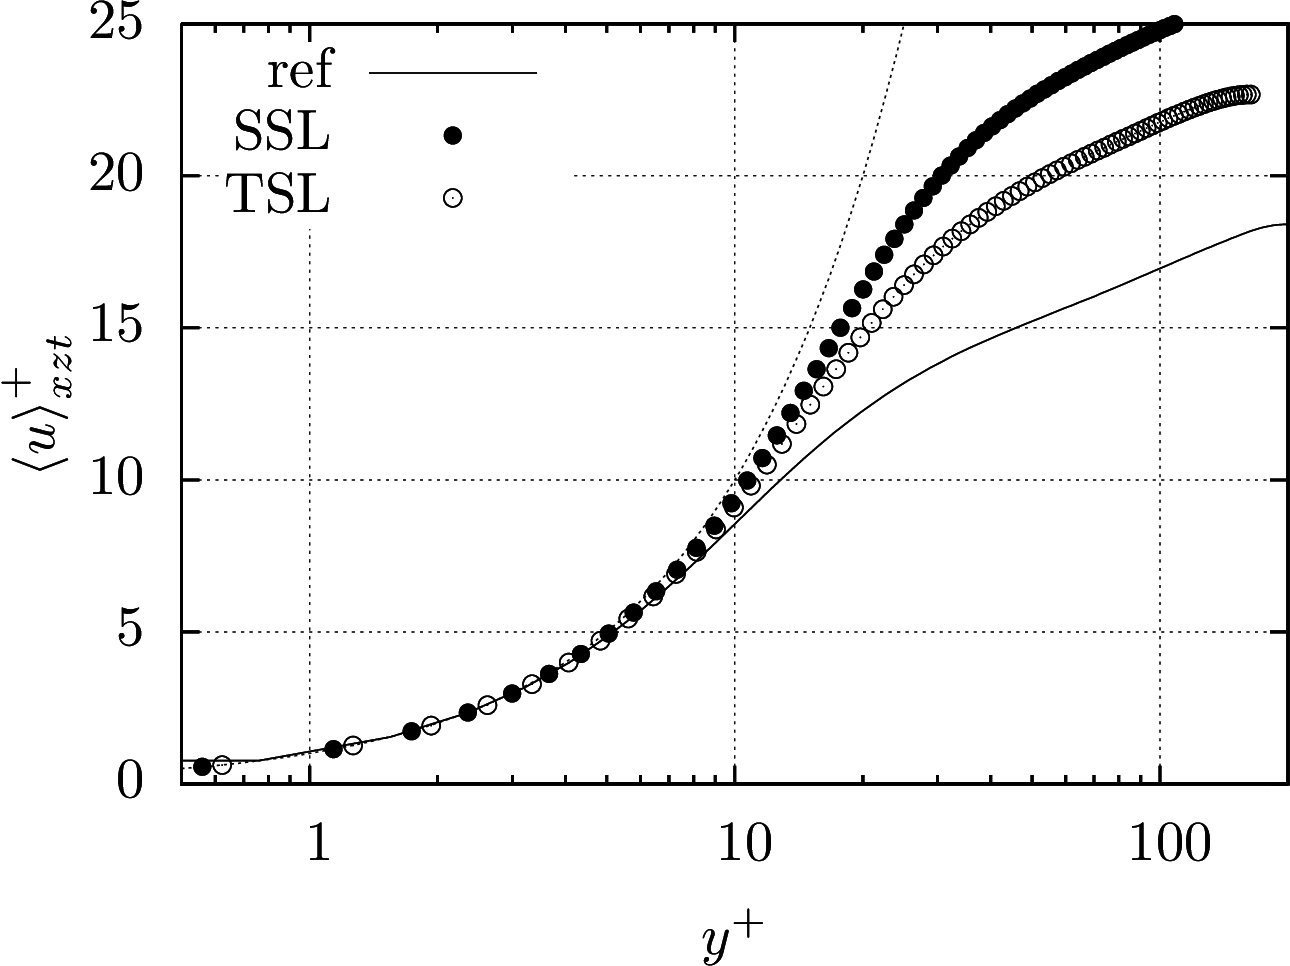
\includegraphics[width=0.5\linewidth]{project/fig/sslmeanprofile.png}
	\caption[Streamwise mean velocity profiles of SSL and reference flow]{Streamwise mean velocity profiles in wall units averaged in $x$-$z$ space, time, and phase ($\overline{U}^{+}\equiv \left<u \right>^{+}_{xzt}$) for \gls{ssl}, \gls{tsl}, the reference flow, and $\overline{U}^{+}=y^{+}$ (dotted line) for comparison \cite{viotti2009}.}
	\label{fig:sslmeanprofile}
\end{figure}

In order to see the differences more clearly, the  \gls{ssl} and refence flow data from Figure~\ref{fig:sslmeanprofile} were digitised using the web app webplotdigitiser. Then a curve fit was implemented and plotted in Figure~\ref{fig:sslmpcf} using an analytical fit for a turbulent plane channel flows given in an unpublished supplement to \cite{chernyshenko2021}. Abnormally, though, when the curve fit given for the mean streamwise velocity was used, the derivative thereof fluctuated much more than expected. Therefore, the curve fit for the second moments of velocity near the wall (root mean square velocity) was trialled instead, which produced much more reasonable derivative whilst also maintaining a good curve fit in and of itself. This latter curve fit is given as
\begin{equation}
	y^{+}  \frac{a\left(y^{+}\right)^2 + by^{+} + c}{q\left(y^{+}\right)^2 + ry^{+} + 1} + p \left( \ln(y^{+}+15)-\ln(15)\right)\label{eq:curvefit}
,\end{equation}
where $a,b,c,p,q,r$ are some coefficients. This function, however, does not guarantee that $\dv{U^{+}}{y^{+}} =1$ at the wall, which would be most accurate. We can see again that at $y^{+}<10$, the curves both fit on the $\overline{U}^{+}=y^{+}$ line. Then there is an area where the two curves diverge, but then, at around $y^{+}>60$, the gradients $\dv{\overline{U}^{+}}{y^{+}} $ seem to look fairly similar and in fact become negligible. This can in fact be seen in Figure~\ref{fig:sslmpdiff}, where the squares of the derivatives of the curvefits found using Equation~\eqref{eq:curvefit} were plotted for the \gls{ssl} and reference flows. The dissipation is equal to the integral of this derivative from 0 to infinity, however as we can see the area under the curve is comparatively negligible at $y^{+}>60$. This, as \textcite{viotti2009} had done, lead us to conjecture that the logarithmic portion of the \gls{ssl} mean velocity profile was the same as that of the reference flow but with an extra vertical shift.

Therefore, 

\begin{figure}[htbp]
	\centering
	\subfigure[Curve fits.]{
		\label{fig:sslmpcf}
        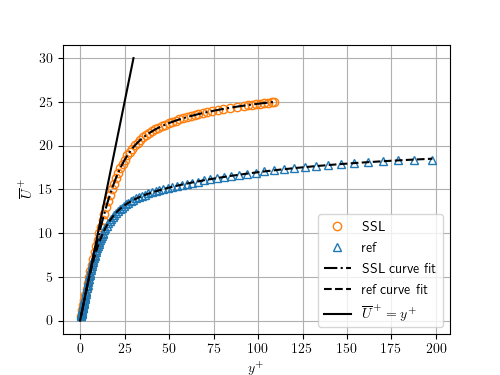
\includegraphics[width=0.485\linewidth]{project/fig/sslmeanprofilelin.png}}
	\subfigure[Estimated logarithmic profiles.]{
		\label{fig:sslmpest}
		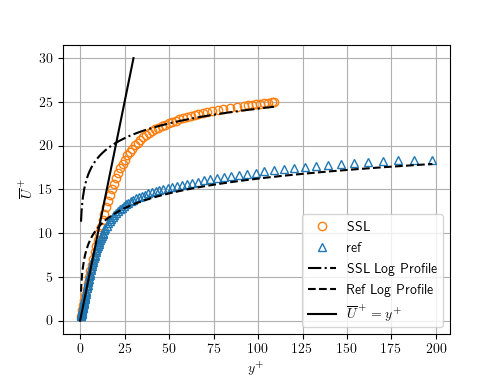
\includegraphics[width=0.485\linewidth]{project/fig/sslmeanprofileest.png}}
		\caption[Mean streamwise velocity profiles of SSL and reference flows, and analytical approximations thereof]{Both plots show data on the mean streamwise velocity profiles of \gls{ssl} (orange-circle) and the reference flow (blue-triangles) which were digitised from \textcite{viotti2009} (shown in Figure~\ref{fig:sslmeanprofile} and plotted on a linear scale, as well as $\overline{U}^+=y^+$ (solid-line). }
	\label{fig:sslmplin}
\end{figure}

\begin{figure}[htbp]
	\centering
	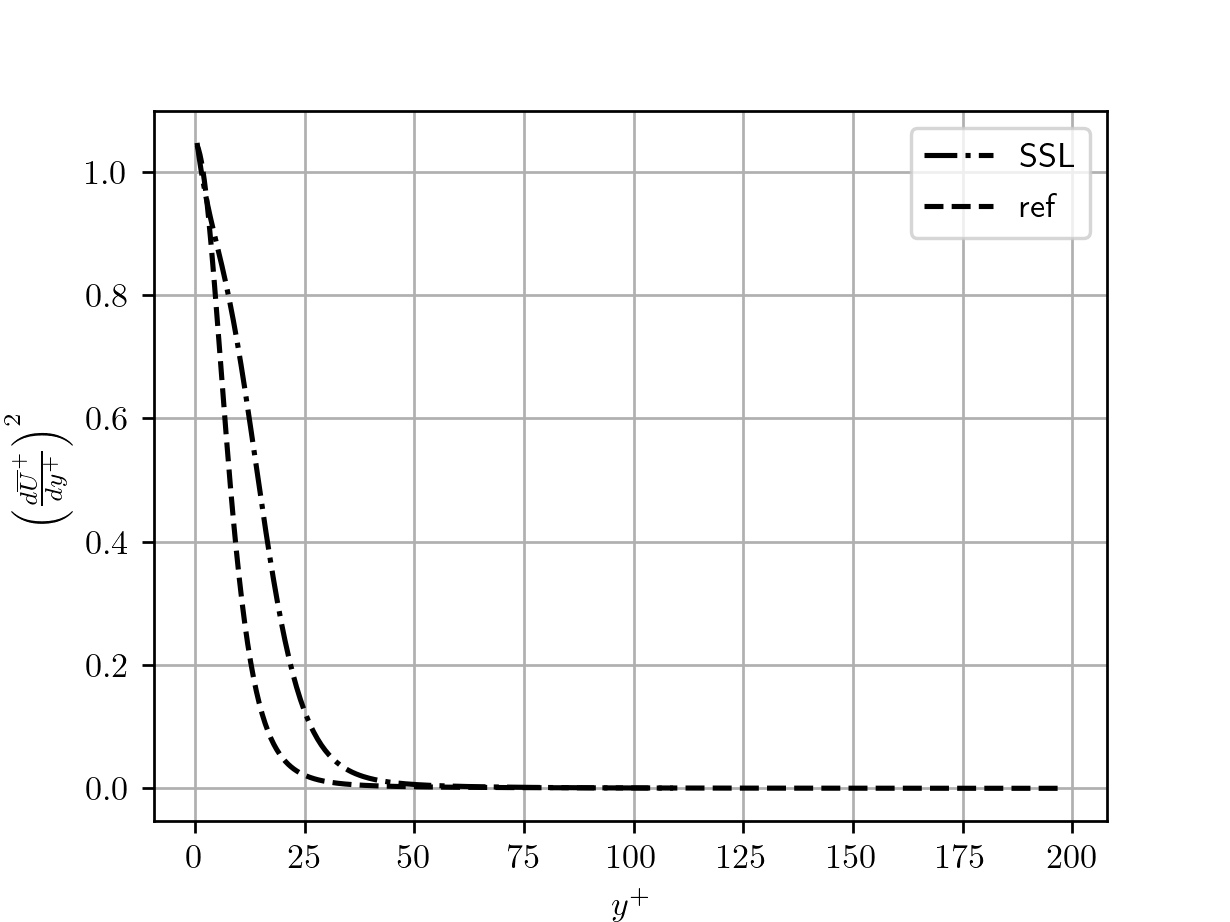
\includegraphics[width=0.485\linewidth]{project/fig/sslmeandiff.png}
	\caption[Mean streamwise shear profile squared of SSL and reference flows]{The squared mean streamwise shear profiles of \gls{ssl} (dot-dash), and reference (dash) flows, i.e. the squared derivative of mean streamwise velocity profiles $\dv{\overline{U}^{+}}{y^{+}} $ obtained using Equation~\eqref{eq:curvefit} for $\overline{U}^{+}$, which is shown in Figure~\ref{fig:sslmpcf}.}
	\label{fig:sslmpdiff}
\end{figure}
In seeing that the logarithmic portion of the mean velocity profilethe complete similarity at $y^{+}<10$, and 
